\documentclass[10pt,twocolumn]{article}

% ============================================================
%  Plantilla conforme al Anexo A — Formato del Informe Técnico
%  Teoría de la Computación — FaCENA, UNNE — 2026
% ============================================================

\usepackage{fontspec}
\setmainfont{Liberation Serif} % equivalente métrico de Times New Roman

\usepackage[left=2.5cm,right=2.5cm,top=2.5cm,bottom=2.0cm]{geometry}
\usepackage{graphicx}
\usepackage{caption}
\usepackage{amsmath,amssymb}
\usepackage{xcolor}
\usepackage{listings}
\usepackage{tabularx}
\usepackage{booktabs}
\usepackage{multicol}
\usepackage[hidelinks]{hyperref}
\usepackage{enumitem}
\usepackage{needspace}

\captionsetup{font=small,labelfont=bf}
\renewcommand{\figurename}{Fig.}
\renewcommand{\tablename}{Tabla}
\renewcommand{\lstlistingname}{Listado}

% Estilo de listados de código
\definecolor{codebg}{HTML}{F5F5F5}
\definecolor{codecomment}{HTML}{6A9955}
\definecolor{codekeyword}{HTML}{0000AA}
\lstset{
  basicstyle=\ttfamily\footnotesize,
  backgroundcolor=\color{codebg},
  commentstyle=\color{codecomment}\itshape,
  keywordstyle=\color{codekeyword}\bfseries,
  numbers=left,
  numberstyle=\tiny,
  numbersep=5pt,
  frame=single,
  breaklines=true,
  showstringspaces=false,
  tabsize=2,
  columns=fullflexible,
}

\lstdefinelanguage{maplang}{
  keywords={MAP, ROOM, CONNECT, SIZE, TYPE, EXITS, ENEMY, LEVEL, ITEM, NPC, via},
  morecomment=[l]{//},
  morestring=[b]",
  sensitive=true,
}

\setlength{\columnsep}{0.7cm}
\pagenumbering{gobble} % Anexo A: no numerar las páginas en el PDF final

\title{\textbf{\fontsize{16}{19}\selectfont MapLang: Diseño e Implementación de un
Analizador Léxico-Sintáctico para la Descripción Textual de Mapas de
Videojuegos de Tipo \textit{Dungeon-Crawler}}}

\author{
\footnotesize
L.\ Riveros$^{a}$, M.\ Riveros$^{a}$, S.\ Scetti$^{a}$, S.\ Turtola$^{a}$\\[2pt]
\footnotesize $^{a}$ Facultad de Ciencias Exactas y Naturales y Agrimensura, Universidad Nacional del Nordeste\\
\footnotesize Teoría de la Computación, 4.\textsuperscript{o} año, Licenciatura en Sistemas de Información\\
\footnotesize Grupo 50 --- Proyecto SIC-UNNE
}
\date{}

\begin{document}
\twocolumn[
  \begin{@twocolumnfalse}
    \maketitle
    \begin{abstract}
    \noindent\small
    Se presenta el diseño y la implementación de MapLang, un lenguaje de
    dominio específico orientado a la descripción textual, no ambigua, de
    mapas de videojuegos del género \textit{dungeon-crawler}. Se define
    formalmente una gramática libre de contexto de veinte producciones que
    satisface la condición LL(1), lo cual habilita la construcción de un
    analizador léxico manual y un analizador sintáctico descendente
    recursivo, ambos implementados en Python. El sistema construye un
    Árbol Sintáctico Abstracto tipado, aplica un conjunto de validaciones
    semánticas adicionales (límites del mapa, unicidad de coordenadas,
    referencias válidas entre salas) y genera, a partir del árbol, una
    representación gráfica del mapa mediante la biblioteca matplotlib. Se
    diseñaron catorce casos de prueba (ocho válidos y seis inválidos,
    incluyendo casos límite) que se validan mediante una suite automatizada
    de cincuenta y dos pruebas unitarias y de integración. Los resultados
    muestran que el analizador reconoce correctamente el lenguaje definido,
    rechaza entradas mal formadas con mensajes orientados al usuario, y
    permite una recuperación básica de errores que posibilita reportar
    múltiples fallos sintácticos en una sola pasada.
    \end{abstract}
    \vspace{0.4cm}
  \end{@twocolumnfalse}
]

% ============================================================
\section{Introducción}
% ============================================================

Los lenguajes de dominio específico (DSL) permiten reducir la brecha entre
una necesidad de comunicación técnica y su representación procesable por
una máquina, restringiendo el vocabulario y la sintaxis disponibles a un
problema acotado \cite{aho2006compilers}. En el desarrollo de videojuegos,
la descripción de niveles y mapas constituye una tarea recurrente que en la
mayoría de las herramientas comerciales se resuelve mediante editores
gráficos propietarios, lo cual dificulta el versionado en sistemas de
control de cambios, la generación procedural de contenido y la
colaboración basada en texto plano entre diseñadores.

Este trabajo presenta \textbf{MapLang}, un DSL textual para describir mapas
de tipo \textit{dungeon-crawler}: estructuras de habitaciones conectadas
entre sí, cada una con un conjunto de atributos (tipo de sala, salidas
disponibles, enemigo presente, nivel de dificultad, ítem y personaje no
jugable). El objetivo del trabajo es doble: por un lado, especificar
formalmente una gramática no ambigua para este lenguaje y, por otro,
construir un analizador léxico-sintáctico completo --- con manejo de
errores, generación de AST y una salida visual --- que permita validar
cadenas de entrada y demostrar de forma tangible los conceptos de la
Teoría de la Computación abordados en la asignatura: gramáticas formales,
autómatas, derivaciones, ambigüedad y técnicas de parsing.

La motivación de elegir este dominio responde a varios criterios. En
primer lugar, su \textbf{riqueza gramatical}: el lenguaje requiere
estructuras anidadas (un mapa contiene salas, cada sala contiene
atributos), listas (las salidas de una sala) y recursividad, lo cual
permite ejercitar una gramática no trivial sin recurrir a artificios. En
segundo lugar, su \textbf{potencial visual}: a diferencia de un DSL
puramente textual, MapLang permite renderizar el AST resultante como una
imagen del mapa, lo que aporta una demostración de alto impacto durante la
exposición oral. Finalmente, existe \textbf{aplicabilidad real}: editores
como Tiled Map Editor o el sistema de \textit{tilemaps} de Godot resuelven
problemas análogos en la industria.

El resto del informe se organiza como sigue. La Sección 2 repasa los
conceptos teóricos de gramáticas formales y autómatas empleados como marco
de referencia. La Sección 3 presenta el diseño formal de la gramática de
MapLang. La Sección 4 describe la arquitectura de la implementación. La
Sección 5 expone los casos de prueba y resultados obtenidos. La Sección 6
discute las dificultades encontradas y posibles extensiones. La Sección 7
concluye el trabajo.

% ============================================================
\section{Marco Teórico}
% ============================================================

\subsection{Gramáticas formales}

Siguiendo la formalización clásica, una gramática formal se define como
una cuaterna $G = (N, T, P, S)$, donde $N$ es un conjunto finito de
símbolos no terminales, $T$ un conjunto finito de símbolos terminales con
$N \cap T = \emptyset$, $P$ un conjunto finito de producciones de la forma
$\alpha \rightarrow \beta$, y $S \notin N \cup T$ el símbolo distinguido
\cite{teoria_computacion_cattedra}. El lenguaje generado por $G$ se define
como
\[
L(G) = \{\, \omega \in T^{*} \mid S \overset{*}{\Rightarrow} \omega \,\}.
\]
La jerarquía de Chomsky clasifica a las gramáticas en cuatro tipos según
la forma de sus producciones, desde las gramáticas sin restricción (Tipo
0) hasta las gramáticas regulares (Tipo 3). El lenguaje MapLang se
especifica mediante una \textbf{Gramática Libre de Contexto (GLC, Tipo
2)}: todas sus producciones tienen la forma $A \rightarrow \omega$ con
$A \in N$ y $\omega \in (N \cup T)^{*}$, sin restricción de contexto sobre
los símbolos adyacentes.

\subsection{Derivaciones, árboles y ambigüedad}

Una \textit{derivación} es la secuencia de formas sentenciales obtenida al
reescribir sucesivamente un no terminal mediante las producciones de $G$,
comenzando en $S$. Una \textit{derivación por izquierda} reescribe en cada
paso el símbolo no terminal más a la izquierda de la forma sentencial
actual. Una gramática libre de contexto es \textbf{ambigua} si y solo si
existe al menos una sentencia de $L(G)$ con dos o más derivaciones por
izquierda distintas, lo cual se traduce en dos árboles de derivación
estructuralmente diferentes (o estructuralmente iguales pero con distintos
rótulos en sus nodos internos) \cite{teoria_computacion_cattedra}. Esta
definición es la que se emplea en la Sección 3.5 para argumentar la no
ambigüedad de la gramática de MapLang.

\subsection{Autómatas de estados finitos y su rol en el lexer}

El analizador léxico de MapLang puede modelarse conceptualmente como un
autómata de estados finitos determinístico
$M = (Q, \Sigma, \delta, q_0, F)$ que recorre el código fuente carácter a
carácter, donde cada ``categoría de token'' corresponde a una clase de
caminos de aceptación distinta dentro del diagrama de estados implícito en
la función \texttt{tokenize} (Sección 4.1). Si bien la implementación no
instancia una tabla de transición explícita --- por simplicidad y
legibilidad del código se opta por una implementación manual basada en
inspección de caracteres ---, el comportamiento es funcionalmente
equivalente al de un AEF determinístico: cada decisión depende únicamente
del carácter actual y de un estado interno acotado (por ejemplo, ``dentro de
una cadena'', ``leyendo un identificador'').

\subsection{Técnicas de parsing}

Para el reconocimiento sintáctico se evaluaron tres estrategias: parser
descendente recursivo, parser LL(1) con tabla, y parsers ascendentes
(SLR/LALR). Se seleccionó el \textbf{parser descendente recursivo}, dado
que la gramática de MapLang es LL(1) (ver Sección 3.6) y esta técnica
ofrece la ventaja de una correspondencia directa y legible entre cada
no-terminal de la gramática y una función del programa, facilitando tanto
la implementación manual como el control granular sobre el reporte de
errores --- un requisito explícito del trabajo.

% ============================================================
\section{Diseño de la Gramática}
% ============================================================

\subsection{Clase gramatical}

La gramática definida para MapLang es una Gramática Libre de Contexto.
Tras el análisis de los conjuntos FIRST y FOLLOW (Sección 3.6), se
verificó que satisface la condición LL(1), lo que permite la
implementación de un parser descendente recursivo sin necesidad de
\textit{backtracking}.

\subsection{Notación BNF}

La Tabla \ref{tab:produc} presenta las veinte producciones que definen la
gramática completa de MapLang.

\begin{table*}[t]
\centering
\caption{Producciones BNF de la gramática de MapLang.}
\label{tab:produc}
\small
\begin{tabularx}{\textwidth}{l l X}
\toprule
\textbf{\#} & \textbf{No terminal} & \textbf{Producción} \\
\midrule
P1  & \texttt{<programa>}      & \texttt{<programa> ::= <mapa>+} \\
P2  & \texttt{<mapa>}           & \texttt{<mapa> ::= "MAP" <cadena> "SIZE" <dimension> "\{" <cuerpo> "\}"} \\
P3  & \texttt{<cuerpo>}          & \texttt{<cuerpo> ::= <declaracion>+} \\
P4  & \texttt{<declaracion>}      & \texttt{<declaracion> ::= <sala> | <conexion>} \\
P5  & \texttt{<sala>}              & \texttt{<sala> ::= "ROOM" "(" <entero\_pos> "," <entero\_pos> ")" <atributo>+} \\
P6  & \texttt{<atributo>}          & \texttt{<atributo> ::= <tipo\_sala> | <salidas> | <enemigo> | <nivel> | <item> | <npc>} \\
P7  & \texttt{<tipo\_sala>}         & \texttt{<tipo\_sala> ::= "TYPE" "=" <tipo\_valor>} \\
P8  & \texttt{<tipo\_valor>}        & \texttt{<tipo\_valor> ::= "entrada" | "pasillo" | "combate" | "tesoro" | "jefe" | "tienda" | "trampa"} \\
P9  & \texttt{<salidas>}            & \texttt{<salidas> ::= "EXITS" "=" "[" <lista\_dir> "]"} \\
P10 & \texttt{<lista\_dir>}          & \texttt{<lista\_dir> ::= <direccion> ("," <direccion>)*} \\
P11 & \texttt{<direccion>}            & \texttt{<direccion> ::= "norte" | "sur" | "este" | "oeste" | "arriba" | "abajo"} \\
P12 & \texttt{<enemigo>}               & \texttt{<enemigo> ::= "ENEMY" "=" <identificador>} \\
P13 & \texttt{<nivel>}                  & \texttt{<nivel> ::= "LEVEL" "=" <entero\_pos>} \\
P14 & \texttt{<item>}                    & \texttt{<item> ::= "ITEM" "=" <identificador>} \\
P15 & \texttt{<npc>}                      & \texttt{<npc> ::= "NPC" "=" <identificador>} \\
P16 & \texttt{<conexion>}                  & \texttt{<conexion> ::= "CONNECT" "(" <entero\_pos> "," <entero\_pos> ")" "->" "(" <entero\_pos> "," <entero\_pos> ")" [ "via" <cadena> ]} \\
P17 & \texttt{<dimension>}                  & \texttt{<dimension> ::= <entero\_pos> "x" <entero\_pos>} \\
P18 & \texttt{<cadena>}                      & \texttt{<cadena> ::= '"' <caracter>* '"'} \\
P19 & \texttt{<identificador>}                & \texttt{<identificador> ::= [a-zA-Z\_][a-zA-Z0-9\_]*} \\
P20 & \texttt{<entero\_pos>}                    & \texttt{<entero\_pos> ::= [0-9]+} \\
\bottomrule
\end{tabularx}
\end{table*}

\subsection{Justificación de las decisiones de diseño}

\textbf{Palabras clave distintivas por atributo.} La producción P6 admite
seis alternativas (\texttt{TYPE}, \texttt{EXITS}, \texttt{ENEMY},
\texttt{LEVEL}, \texttt{ITEM}, \texttt{NPC}), cada una identificada por una
palabra reservada única. Esta decisión elimina cualquier conflicto de
predicción: $\mathrm{FIRST}$ de cada alternativa es un conjunto unitario y
disjunto del resto, por lo que el parser puede elegir la producción
correcta observando un único token de \textit{lookahead}.

\textbf{Orden libre de atributos.} Inicialmente se consideró una gramática
que fijara el orden de aparición de los atributos dentro de una
\texttt{ROOM} (por ejemplo, \texttt{TYPE} antes que \texttt{EXITS}). Se
descartó esta alternativa porque incrementaba artificialmente el número de
producciones sin aportar expresividad, y porque impondría al usuario del
lenguaje una restricción arbitraria. La producción P6, al permitir que
\texttt{<atributo>} se repita en cualquier orden mediante la clausura
positiva de P5, resuelve este problema sin introducir ambigüedad (ver
Sección 3.5).

\textbf{Conexión con etiqueta opcional.} La cláusula
\texttt{[ "via" <cadena> ]} de P16 introduce la única parte opcional de
toda la gramática. Se decidió expresarla como una elección entre presencia
y ausencia (en lugar de duplicar la producción \texttt{<conexion>} en dos
alternativas) porque esta forma simplifica la función
\texttt{parse\_conexion} del parser (Sección 4.2) a una única
verificación condicional, y porque la decisión es LL(1) segura: el token
\texttt{"via"} no pertenece a $\mathrm{FOLLOW}(\texttt{<conexion>})$ (ver
Sección 3.6).

\textbf{Enteros no negativos.} Tras el Avance 1, se introdujo expl\'icitamente
\texttt{<entero\_pos>} en lugar de un \texttt{<entero>} genérico, reforzando
que coordenadas y niveles de dificultad deben ser valores no negativos.
Esto no cambia el conjunto de cadenas reconocidas por el lexer (que sólo
tokeniza secuencias de dígitos, intrínsecamente no negativas) pero clarifica
la intención semántica de la producción en la documentación de la
gramática.

\subsection{Recursividad y anidamiento}

La recursividad de la gramática se manifiesta en tres producciones: P1
(\texttt{<programa> ::= <mapa>+}, permite un número arbitrario de mapas en
un mismo programa), P3 (\texttt{<cuerpo> ::= <declaracion>+}, un número
arbitrario de salas y conexiones por mapa) y P10
(\texttt{<lista\_dir> ::= <direccion> ("," <direccion>)*}, listas de
longitud arbitraria de direcciones de salida). El anidamiento se observa en
que un \texttt{<mapa>} contiene un \texttt{<cuerpo>} que contiene
\texttt{<sala>}, la cual a su vez contiene múltiples \texttt{<atributo>}; y
en que un \texttt{<atributo>} de tipo \texttt{<salidas>} contiene una
\texttt{<lista\_dir>}.

\subsection{Justificación de no ambigüedad}

De acuerdo a la definición de ambigüedad expuesta en la Sección 2.2, una
GLC es ambigua si y solo si alguna sentencia de su lenguaje admite dos
derivaciones por izquierda distintas. Se argumenta la no ambigüedad de
MapLang por inspección de cada producción con más de una alternativa:

\begin{itemize}[leftmargin=*,itemsep=1pt]
  \item \textbf{P4} (\texttt{<sala>} | \texttt{<conexion>}): las
  alternativas comienzan, respectivamente, con las palabras clave
  \texttt{ROOM} y \texttt{CONNECT}, mutuamente excluyentes.
  \item \textbf{P6} (las seis variantes de \texttt{<atributo>}): cada una
  comienza con una palabra clave distinta, como se discutió en 3.3.
  \item \textbf{P8} y \textbf{P11} (\texttt{<tipo\_valor>} y
  \texttt{<direccion>}): cada alternativa es un terminal literal distinto;
  no existe superposición léxica entre ellos porque el lexer asigna a cada
  palabra reservada una única categoría de token (Sección 4.1).
\end{itemize}

Dado que en ningún punto de una derivación existe más de una producción
aplicable para un mismo prefijo de entrada, se concluye que toda sentencia
de $L(G)$ posee una única derivación por izquierda y, por lo tanto, un
único árbol de derivación: la gramática \textbf{no es ambigua}. Esta
propiedad se verifica empíricamente en la prueba automatizada
\texttt{test\_same\_input\_always\_same\_ast\_structure} (Sección 5.3).

\subsection{Verificación de la condición LL(1)}

Una gramática es LL(1) si para cada no terminal con más de una producción,
los conjuntos $\mathrm{FIRST}$ de cada alternativa son disjuntos entre sí
y, en caso de que alguna alternativa derive $\lambda$, dicho conjunto es
también disjunto de $\mathrm{FOLLOW}$ del no terminal. Para MapLang:

\begin{itemize}[leftmargin=*,itemsep=1pt]
\item $\mathrm{FIRST}(\texttt{<sala>}) = \{\texttt{ROOM}\}$,
$\mathrm{FIRST}(\texttt{<conexion>}) = \{\texttt{CONNECT}\}$: disjuntos.
\item $\mathrm{FIRST}(\texttt{<tipo\_sala>}) = \{\texttt{TYPE}\}$,
$\mathrm{FIRST}(\texttt{<salidas>}) = \{\texttt{EXITS}\}$,
$\mathrm{FIRST}(\texttt{<enemigo>}) = \{\texttt{ENEMY}\}$,
$\mathrm{FIRST}(\texttt{<nivel>}) = \{\texttt{LEVEL}\}$,
$\mathrm{FIRST}(\texttt{<item>}) = \{\texttt{ITEM}\}$,
$\mathrm{FIRST}(\texttt{<npc>}) = \{\texttt{NPC}\}$: los seis conjuntos son
disjuntos entre sí.
\item Para la parte opcional de P16, $\mathrm{FOLLOW}(\texttt{<conexion>})
= \mathrm{FIRST}(\texttt{<declaracion>}) \cup \{\texttt{"\}"}\} =
\{\texttt{ROOM}, \texttt{CONNECT}, \texttt{"\}"}\}$. Como
\texttt{"via"} $\notin \mathrm{FOLLOW}(\texttt{<conexion>})$, la decisión
de tomar o no la cláusula opcional se resuelve con un único token de
\textit{lookahead} sin ambigüedad.
\end{itemize}

No se presenta el cálculo completo de FIRST/FOLLOW para las veinte
producciones por razones de espacio; el razonamiento anterior cubre los
únicos puntos de decisión no triviales de la gramática --- el resto de las
producciones no requiere elección entre alternativas (son únicas) o se
resuelve trivialmente por la palabra clave inicial.

\subsection{Ejemplo de cadena válida e inválida}

\begin{lstlisting}[language=maplang,caption={Cadena válida: la «Mazmorra del Dragón».}]
MAP "Mazmorra_del_Dragon" SIZE 8x8 {
  ROOM(0,0) TYPE=entrada EXITS=[este,sur]
  ROOM(1,0) TYPE=combate ENEMY=goblin LEVEL=2
  ROOM(2,0) TYPE=tesoro ITEM=pocion_vida
  ROOM(3,0) TYPE=jefe ENEMY=dragon LEVEL=10
  CONNECT (0,0)->(1,0) via "corredor_este"
  CONNECT (1,0)->(2,0) via "puerta_madera"
  CONNECT (2,0)->(3,0) via "puerta_secreta"
}
\end{lstlisting}

\begin{lstlisting}[language=maplang,caption={Cadena inválida: faltan paréntesis y coordenadas.}]
MAP "Mapa_Roto" SIZE abc {
  ROOM(0,0 TYPE=entrada
  ROOM(1,) TYPE=combate
  CONNECT (0,0)-> via "x"
}
\end{lstlisting}

% ============================================================
\section{Implementación}
% ============================================================

La implementación se realizó en Python 3.12, por su legibilidad, su amplio
ecosistema de bibliotecas y su facilidad para integrar la visualización del
AST y del mapa generado. El sistema se organiza en cinco módulos
independientes (Fig.~\ref{fig:arq}): \texttt{lexer.py},
\texttt{parser.py}, \texttt{ast\_nodes.py}, \texttt{semantic.py} y
\texttt{renderer.py}, integrados por \texttt{main.py}.

\begin{figure}[t]
\centering
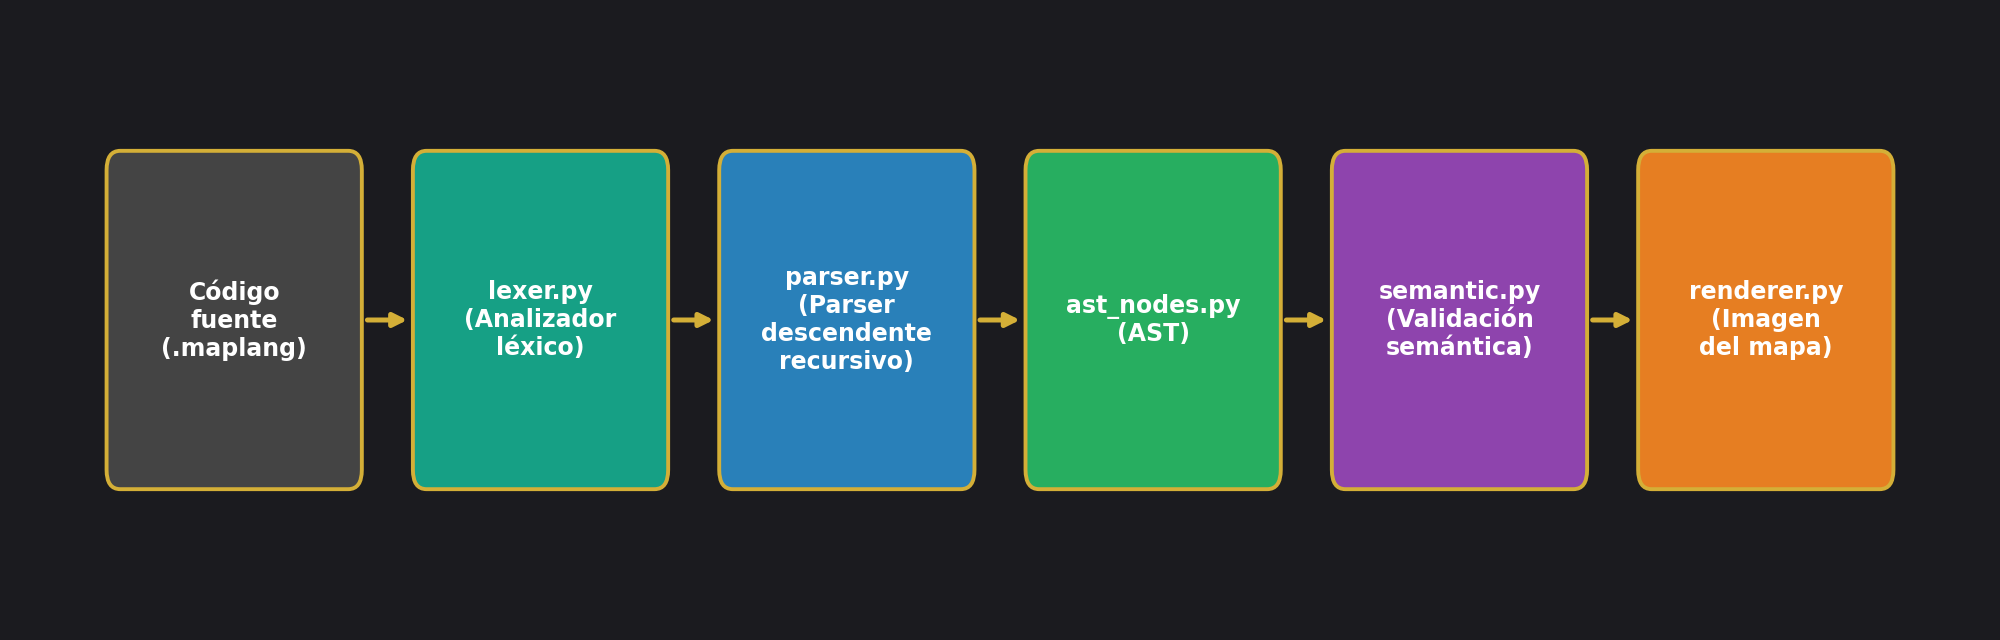
\includegraphics[width=\linewidth]{figs/fig_arquitectura.png}
\caption{Arquitectura modular del sistema MapLang.}
\label{fig:arq}
\end{figure}

\subsection{Analizador léxico}

El lexer (\texttt{lexer.py}) se implementó de forma manual --- sin
bibliotecas como Flex, PLY o ANTLR --- recorriendo el código fuente
carácter a carácter. Cada categoría de token se reconoce mediante
inspección directa de prefijos: cadenas delimitadas por comillas dobles,
secuencias de dígitos (posiblemente seguidas de \texttt{x} y otra secuencia
de dígitos, lo que se interpreta como literal de dimensión SIZE), e
identificadores que se clasifican retroactivamente como palabra clave,
valor de tipo de sala, dirección, o identificador genérico según
pertenezcan o no a los conjuntos \texttt{KEYWORDS}, \texttt{TYPE\_VALS} o
\texttt{DIRECTIONS}. La Tabla \ref{tab:tokens} resume las categorías de
token reconocidas. Los espacios en blanco y los comentarios de línea
(\texttt{// ...}) se descartan sin generar token. Cada token registra
línea y columna de origen, información reutilizada en el reporte de
errores tanto léxicos como sintácticos.

\begin{table}[h]
\centering
\caption{Categorías de token del lexer de MapLang.}
\label{tab:tokens}
\small
\begin{tabularx}{\linewidth}{l X}
\toprule
\textbf{Categoría} & \textbf{Ejemplos} \\
\midrule
KEYWORD    & MAP, ROOM, CONNECT, TYPE, EXITS, ENEMY, LEVEL, ITEM, NPC, SIZE, via \\
TYPE\_VAL   & entrada, pasillo, combate, tesoro, jefe, tienda, trampa \\
DIRECTION   & norte, sur, este, oeste, arriba, abajo \\
STRING       & "Mazmorra\_1", "puerta\_madera" \\
SIZE          & 8x8, 10x12, 5x5 \\
INTEGER        & 0, 1, 3, 10, 255 \\
IDENTIFIER      & goblin, espada\_magica, mercader \\
PUNCT            & \{ \} ( ) [ ] = , -> \\
\bottomrule
\end{tabularx}
\end{table}

Ante un carácter no reconocido o una cadena sin cerrar, el lexer lanza una
excepción \texttt{LexError} que incluye número de línea y columna.

\subsection{Analizador sintáctico}

El parser (\texttt{parser.py}) implementa un \textbf{descendente
recursivo}: cada no-terminal de la gramática (Tabla \ref{tab:produc}) se
traduce en un método \texttt{parse\_X} de la clase \texttt{Parser}, que
consume tokens de una lista y construye el nodo de AST correspondiente. El
Listado~\ref{lst:parse_conexion} muestra la implementación de
\texttt{parse\_conexion}, que ilustra la resolución de la parte opcional
discutida en la Sección 3.3 mediante un único \textit{lookahead}.

\begin{lstlisting}[language=Python,caption={Fragmento de \texttt{parse\_conexion} (parte opcional vía LL(1)).},label={lst:parse_conexion}]
etiqueta = None
if self.check_keyword("via"):
    self.advance()
    etiqueta_tok = self.expect_type(
        "STRING", "una cadena (etiqueta)")
    etiqueta = etiqueta_tok.value
\end{lstlisting}

\textbf{Manejo y recuperación de errores.} Ante un token inesperado se
lanza \texttt{ParseError} con línea, columna y un mensaje orientado al
usuario (p.\ ej. \textit{"se esperaba ')' pero se encontró 'TYPE'
(KEYWORD)"}). Cuando se invoca el parser en modo
\texttt{collect\_errors=True}, los errores producidos dentro de
\texttt{<sala>} o \texttt{<conexion>} no abortan el análisis: se registran
y el parser ejecuta una rutina de \textbf{sincronización en modo pánico}
que descarta tokens hasta encontrar el inicio de la siguiente declaración
(\texttt{ROOM}/\texttt{CONNECT}) o el cierre de bloque (\texttt{"\}"}). Esto
permite reportar varios errores sintácticos en una sola ejecución, en lugar
de detenerse en el primero (verificado en
\texttt{test\_multiple\_errors\_recovered}, Sección 5.3).

\subsection{Árbol Sintáctico Abstracto}

El AST se modela en \texttt{ast\_nodes.py} mediante \textit{dataclasses}
de Python (\texttt{Programa}, \texttt{Mapa}, \texttt{Sala},
\texttt{Conexion} y los seis tipos de atributo), lo que provee
automáticamente comparación estructural --- usada extensivamente en los
tests --- y un método \texttt{to\_dict()} para la serialización a JSON. El
sistema admite tres representaciones del AST, todas disponibles desde
\texttt{main.py}: árbol textual indentado en consola, exportación a JSON,
y un diagrama Graphviz (Fig.~\ref{fig:ast}, generado por el módulo
auxiliar \texttt{ast\_graphviz.py}).

\begin{figure}[t]
\centering
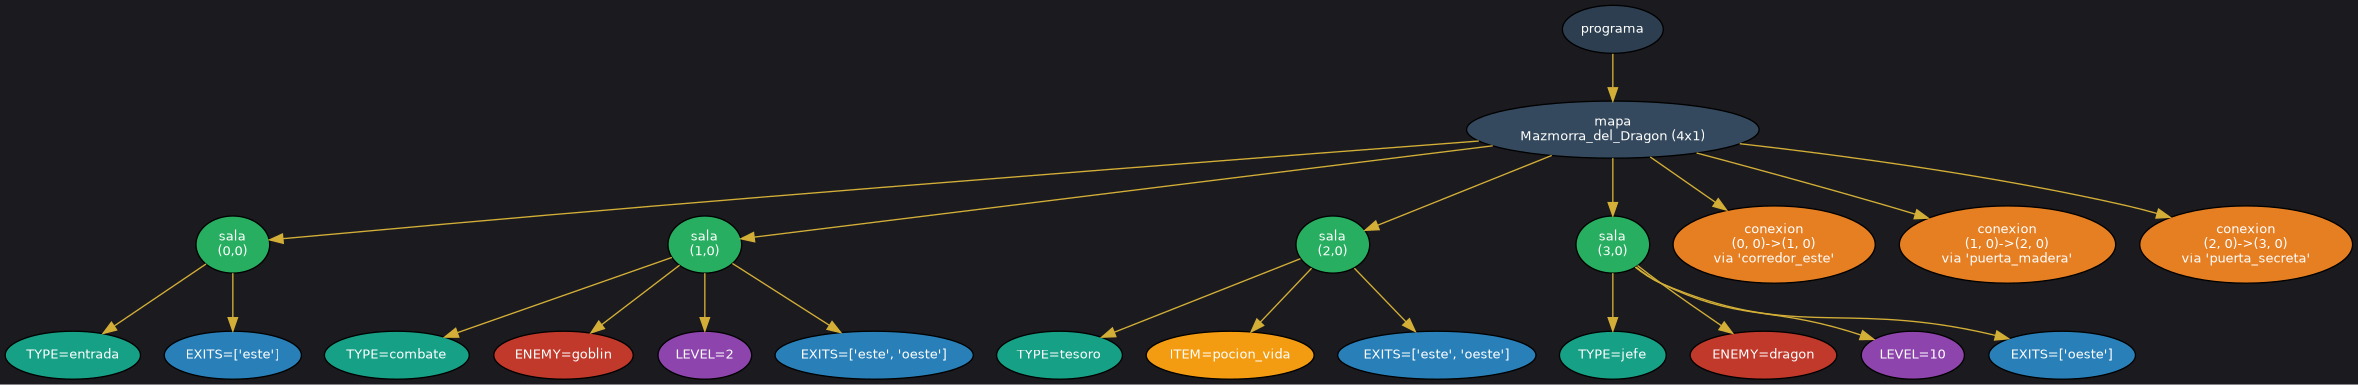
\includegraphics[width=\linewidth]{figs/fig_ast.png}
\caption{AST de la «Mazmorra del Dragón» representado con Graphviz.}
\label{fig:ast}
\end{figure}

\subsection{Validación semántica}

Más allá de lo que una GLC puede expresar convenientemente, se implementó
en \texttt{semantic.py} un recorrido del AST que verifica cuatro reglas
adicionales de buena formación: (S1) las coordenadas de cada sala deben
estar dentro de los límites declarados por \texttt{SIZE}; (S2) no puede
haber dos salas con la misma coordenada; (S3) toda \texttt{CONNECT} debe
referenciar salas existentes; (S4) un atributo no puede repetirse dentro de
la misma sala. Estas reglas dependen del contexto global del mapa --- no de
una única producción --- por lo que se verifican como una etapa posterior
al parseo, análoga al análisis semántico de un compilador convencional.

\subsection{Renderizador}

El módulo \texttt{renderer.py} recorre el AST de un \texttt{Mapa} y
construye, con matplotlib, una grilla donde cada sala se dibuja como una
celda coloreada según su \texttt{TYPE} (Fig.~\ref{fig:mapa}), anotada con
sus atributos, y cada \texttt{CONNECT} como una línea entre los centros de
las salas correspondientes. Esta es la salida visual central del sistema y
el punto de mayor impacto durante la demostración en vivo.

\begin{figure}[t]
\centering
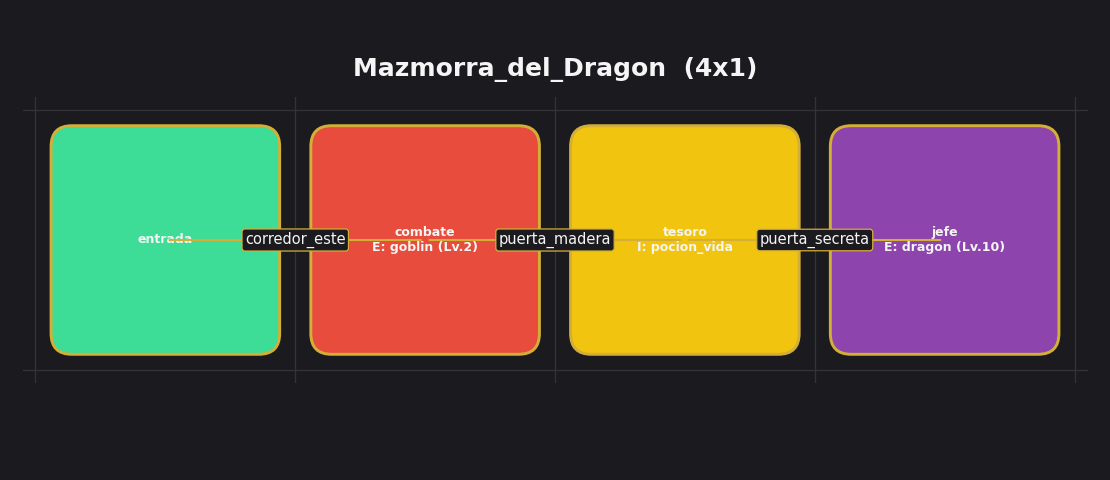
\includegraphics[width=\linewidth]{figs/fig_mapa_dragon.png}
\caption{Renderizado de la «Mazmorra del Dragón» a partir del AST.}
\label{fig:mapa}
\end{figure}

\subsection{Estructura modular y control de versiones}

\begin{lstlisting}[caption={Estructura de archivos del proyecto.}]
src/
  lexer.py         Analizador léxico
  parser.py        Parser descendente recursivo
  ast_nodes.py      Nodos del AST
  semantic.py        Validaciones semánticas
  renderer.py          Renderizador del mapa
  ast_graphviz.py        Exportador a Graphviz
  main.py                  Punto de entrada (CLI)
tests/
  test_lexer.py            20 pruebas unitarias
  test_parser.py            18 pruebas unitarias
  test_semantic.py            10 pruebas unitarias
  test_integration.py           4 pruebas end-to-end
  casos/                           14 archivos .maplang
\end{lstlisting}

% ============================================================
\section{Casos de Prueba y Resultados}
% ============================================================

\subsection{Diseño de los casos}

Se diseñaron catorce casos de prueba almacenados como archivos
\texttt{.maplang} independientes en \texttt{tests/casos/}: ocho casos
válidos (incluyendo un caso límite de dimensión mínima 1×1, múltiples
mapas en un mismo programa, y verificación del orden libre de atributos) y
seis casos inválidos que cubren las tres etapas de validación: errores
léxicos (carácter no reconocido, cadena sin cerrar), errores sintácticos
(paréntesis faltante, coordenada faltante, conexión incompleta, cuerpo
vacío) y errores semánticos (coordenada duplicada, sala fuera de límites,
conexión a sala inexistente). La Tabla~\ref{tab:casos} resume un
subconjunto representativo.

\begin{table}[t]
\centering
\caption{Subconjunto representativo de casos de prueba.}
\label{tab:casos}
\scriptsize
\begin{tabularx}{\linewidth}{X l c}
\toprule
\textbf{Caso} & \textbf{Validación} & \textbf{Result.} \\
\midrule
valido\_01\_lineal           & --- (válido)       & Aceptada \\
valido\_06\_limite\_minimo     & --- (límite 1x1)     & Aceptada \\
valido\_08\_orden\_libre        & --- (válido)           & Aceptada \\
invalido\_01\_caracter           & Léxica                  & Rechazada \\
invalido\_02\_cadena\_sin\_cerrar  & Léxica                    & Rechazada \\
invalido\_03\_sintacticos\_mult.    & Sintáctica (×3)             & Rechazada \\
invalido\_05\_sem\_multiples         & Semántica (×3)                & Rechazada \\
invalido\_06\_cuerpo\_vacio            & Sintáctica                       & Rechazada \\
\bottomrule
\end{tabularx}
\end{table}

\subsection{Ejemplo de salida ante entrada inválida}

Para el caso \texttt{invalido\_05\_\allowbreak errores\_\allowbreak semanticos.maplang}
(una sala duplicada en (0,0), una sala en (5,5) fuera de los límites de un
mapa 2$\times$2, y una conexión hacia la coordenada inexistente (9,9)), el
sistema reporta:

\begin{lstlisting}[caption={Salida real del sistema ante errores semánticos.}]
Error semantico (linea 6): ya existe una sala
  declarada en (0,0) (primera declaracion en
  linea 5)
Error semantico (linea 7): la sala (5,5) esta
  fuera de los limites del mapa 'Test_Semantico'
  (2x2)
Error semantico (linea 8): CONNECT referencia la
  sala de destino (9, 9) que no fue declarada en
  el mapa 'Test_Semantico'
\end{lstlisting}

Los tres errores se reportan en una sola ejecución, cada uno con su número
de línea correspondiente.

\subsection{Suite automatizada de pruebas}

Se implementó una suite de \textbf{52 pruebas automatizadas} con el módulo
\texttt{unittest} de Python, organizada en cuatro archivos
(Tabla~\ref{tab:tests}). Las pruebas de integración ejecutan el pipeline
completo (lexer $\to$ parser $\to$ semántica $\to$ renderer) sobre los
catorce casos de \texttt{tests/casos/}, verificando que los casos válidos
se acepten sin errores y que los inválidos produzcan al menos un error en
la etapa correspondiente. Todas las pruebas finalizan con resultado
\texttt{OK}.

\begin{table}[t]
\centering
\caption{Resumen de la suite de pruebas automatizadas.}
\label{tab:tests}
\scriptsize
\begin{tabularx}{\linewidth}{l X c}
\toprule
\textbf{Archivo} & \textbf{Cobertura} & \textbf{N.} \\
\midrule
test\_lexer.py        & Tokens, errores léxicos               & 20 \\
test\_parser.py        & Producciones válidas/inválidas, recuperación, no-ambigüedad & 18 \\
test\_semantic.py        & Reglas semánticas S1--S4    & 10 \\
test\_integration.py       & Pipeline end-to-end, render & 4 \\
\midrule
\textbf{Total}                & & \textbf{52} \\
\bottomrule
\end{tabularx}
\end{table}

% ============================================================
\section{Discusión y Análisis}
% ============================================================

\textbf{Dificultades encontradas.} El principal desafío de diseño fue
evitar la ambigüedad en la producción de \texttt{<atributo>}: una primera
aproximación que no fijara palabras clave distintivas por atributo
generaría conflictos de predicción al permitir que dos alternativas
compartieran el mismo prefijo. Esto se resolvió --- como se documentó ya
en el Avance 1 --- exigiendo que cada atributo comience con una palabra
reservada exclusiva. Un segundo desafío surgió al decidir la estrategia de
recuperación de errores: una implementación naïve que abortara en el
primer error sintáctico resultaba poco útil para un usuario que comete
varios errores de tipeo en un mismo archivo; la sincronización en modo
pánico hacia el inicio de la siguiente declaración resultó ser la solución
más simple que preserva la mayor cantidad de información útil.

\textbf{Decisiones de diseño relevantes.} Se optó deliberadamente por una
implementación manual del lexer y el parser --- sin herramientas como
ANTLR o PLY --- en línea con el requisito de la cátedra de comprensión y
defensa conceptual de la implementación. Esto exigió mayor cuidado en el
manejo de casos borde (por ejemplo, distinguir un literal \texttt{SIZE}
del tipo \texttt{8x8} de un entero seguido de un identificador que
casualmente comienza con \texttt{x}), pero permitió un control total sobre
los mensajes de error.

\textbf{Posibles extensiones.} El lenguaje actual excluye deliberadamente
la lógica de eventos o \textit{triggers} dentro de las habitaciones, la
herencia entre tipos de sala, y los mapas multi-piso (Avance 1). Una
extensión natural consistiría en agregar un nuevo no-terminal
\texttt{<evento>} anidado dentro de \texttt{<sala>}, lo cual no rompería la
condición LL(1) si se reutiliza el mismo patrón de palabras clave
distintivas. Asimismo, podría incorporarse un análisis de alcanzabilidad
sobre el grafo de conexiones (verificando que todas las salas sean
alcanzables desde la sala de tipo \texttt{entrada}) como una quinta regla
semántica.

% ============================================================
\section{Conclusiones}
% ============================================================

Se diseñó e implementó un analizador léxico-sintáctico completo para
MapLang, un lenguaje de dominio específico para la descripción no ambigua
de mapas de videojuegos. La gramática propuesta, de veinte producciones,
se verificó formalmente como libre de contexto, no ambigua y LL(1), lo que
permitió la construcción de un parser descendente recursivo manual con
manejo y recuperación de errores. El sistema completo --- lexer, parser,
AST, validación semántica y renderizador --- se valida mediante una suite
de 52 pruebas automatizadas y 14 casos de prueba documentados, todos con
resultado correcto. El trabajo permitió aplicar de manera integrada los
conceptos centrales de la asignatura: gramáticas formales, derivaciones,
ambigüedad, autómatas y técnicas de parsing, además de competencias
profesionales de trabajo colaborativo y documentación técnica. Como
aprendizaje de equipo, se destaca la importancia de fijar decisiones de
diseño gramatical (como las palabras clave distintivas) en etapas
tempranas del proyecto, dado que revertirlas una vez avanzada la
implementación del parser resulta costoso.

% ============================================================
\renewcommand{\refname}{Bibliografía}
\begin{thebibliography}{9}

\bibitem{aho2006compilers}
A.~V.~Aho, M.~S.~Lam, R.~Sethi and J.~D.~Ullman,
\textit{Compilers: Principles, Techniques, and Tools}, 2nd ed.
Boston, MA, USA: Addison-Wesley, 2006.

\bibitem{teoria_computacion_cattedra}
Cátedra de Teoría de la Computación,
\textit{Lingüística Matemática y Gramáticas Formales} (material de
cátedra), Facultad de Ciencias Exactas y Naturales y Agrimensura,
Universidad Nacional del Nordeste, 2026.

\bibitem{teoria_automatas_cattedra}
Cátedra de Teoría de la Computación,
\textit{Autómatas de Estados Finitos} (material de cátedra), Facultad de
Ciencias Exactas y Naturales y Agrimensura, Universidad Nacional del
Nordeste, 2026.

\bibitem{tiled}
Tiled Project, ``Tiled Map Editor,'' [En línea]. Available:
\url{https://www.mapeditor.org/}. [Último acceso: 06-2026].

\bibitem{godot}
Godot Engine Community, ``TileMap --- Godot Engine documentation,'' [En
línea]. Available: \url{https://docs.godotengine.org/}. [Último acceso:
06-2026].

\end{thebibliography}

\end{document}
